% CVPR 2025 Paper Template; see https://github.com/cvpr-org/author-kit

\documentclass[10pt,twocolumn,letterpaper]{article}

%%%%%%%%% PAPER TYPE  - PLEASE UPDATE FOR FINAL VERSION
% \usepackage{cvpr}              % To produce the CAMERA-READY version
% \usepackage[review]{cvpr}      % To produce the REVIEW version
\usepackage[pagenumbers]{cvpr} % To force page numbers, e.g. for an arXiv version

% Import additional packages in the preamble file, before hyperref
%
% --- inline annotations
%
\newcommand{\red}[1]{{\color{red}#1}}
\newcommand{\todo}[1]{{\color{red}#1}}
\newcommand{\TODO}[1]{\textbf{\color{red}[TODO: #1]}}
% --- disable by uncommenting  
% \renewcommand{\TODO}[1]{}
% \renewcommand{\todo}[1]{#1}



% It is strongly recommended to use hyperref, especially for the review version.
% hyperref with option pagebackref eases the reviewers' job.
% Please disable hyperref *only* if you encounter grave issues, 
% e.g. with the file validation for the camera-ready version.
%
% If you comment hyperref and then uncomment it, you should delete *.aux before re-running LaTeX.
% (Or just hit 'q' on the first LaTeX run, let it finish, and you should be clear).
\definecolor{cvprblue}{rgb}{0.21,0.49,0.74}
\usepackage[pagebackref,breaklinks,colorlinks,allcolors=cvprblue]{hyperref}
\DeclareMathOperator*{\argmax}{arg\,max}

%%%%%%%%% PAPER ID  - PLEASE UPDATE
\def\paperID{*****} % *** Enter the Paper ID here
\def\confName{CVPR}
\def\confYear{2025}

%%%%%%%%% TITLE - PLEASE UPDATE
\title{Exploring RIC-CNN for rotation dependent images}

%%%%%%%%% AUTHORS - PLEASE UPDATE
\author{CHAN, Chun Yu\\
{\tt\small cychandp@connect.ust.hk}
% For a paper whose authors are all at the same institution,
% omit the following lines up until the closing ``}''.
% Additional authors and addresses can be added with ``\and'',
% just like the second author.
% To save space, use either the email address or home page, not both
\and
FUNG, Hei Yuen\\
{\tt\small hyfungaj@connect.ust.hk}
\and
HE, Ka Sing\\
{\tt\small ksheaa@connect.ust.hk}
}


\begin{document}
\maketitle
\begin{abstract}
Convolutional Neural Networks (CNNs) have demonstrated remarkable performance in various computer vision tasks, attributed to their ability to learn hierarchical features and their translation equivariance. However, standard CNNs lack rotational invariance, leading to performance degradation with rotated objects. While Rotation-Invariant Convolutional Neural Networks (RIC-CNNs) address this, they exhibit limitations in discriminating between rotationally symmetric objects with distinct meanings at different orientations (e.g., '6' and '9'). This limitation, as noted in Mo et al. (2022), can hinder performance in scenarios where such distinctions are crucial. In this work, we explore combining the rotational invariance of RIC-CNNs with the discriminative power of standard CNNs.  Specifically, we investigate several approaches to integrate these architectures, aiming to achieve robust performance on both rotated and non-rotated image datasets. We evaluate our approaches on the MNIST and Traffic Signs datasets, demonstrating improved performance and robustness compared to using either CNNs or RIC-CNNs alone.
\end{abstract}    
\section{Introduction}
\label{sec:intro}

Convolutional Neural Networks (CNNs) have achieved state-of-the-art results in numerous computer vision tasks, owing to their ability to learn hierarchical features and their translation equivariance. However, standard CNNs are inherently sensitive to image rotations, leading to degraded performance when processing rotated images.

%-------------------------------------------------------------------------
\subsection{Deficiencies of CNNs and the Role of Rotational Invariance}

The lack of rotational invariance in CNNs necessitates the use of data augmentation techniques, where training datasets are expanded with rotated versions of existing images. While this can improve performance, it introduces computational overhead and requires careful tuning to determine the appropriate number of rotated versions. To address this, Rotation-Invariant Convolutional Neural Networks (RIC-CNNs) \cite{mo2022riccnnrotationinvariantcoordinateconvolutional} have been proposed, utilizing rotation-invariant coordinate systems to achieve invariance to arbitrary rotations.

\subsection{Limitations of RIC-CNNs and the Need for Equivariance}

While RIC-CNNs effectively handle rotated images, their strict rotational invariance can be a limitation. In scenarios where distinguishing between rotated versions of objects is crucial (e.g., '6' vs. '9'), RIC-CNNs may struggle. In such cases, rotational equivariance – where feature maps transform in the same way as the input image – is desirable to preserve rotational information.

\subsection{Our Hybrid Approach}
To balance the strengths and weaknesses of CNNs and RIC-CNNs, we propose a hybrid approach that combines both architectures. This allows us to leverage the discriminative power of CNNs for rotation-sensitive tasks while benefiting from the robustness of RIC-CNNs to handle general image rotations. We explore several integration strategies to effectively fuse features from both networks.

%-------------------------------------------------------------------------
\subsection{Contributions}
Our contributions include:
\begin{itemize}
    \item Developing hybrid CNN-RIC-CNN architectures for improved performance on both rotated and non-rotated images.
    \item Evaluating the proposed methods on the MNIST and Traffic Signs datasets.

\end{itemize}


\section{Related Works}
\label{sec:related}

In this section, we focus on Rotation-Invariant Convolutional Neural Networks (RIC-CNNs).

\subsection{Rotation-Invariant Coordinate Convolutional Neural Network}

Mo and Zhao (2022) introduce the \emph{Rotation-Invariant Coordinate Convolution} (RIC-C) to embed structural rotation invariance into the convolution operation.  We first recall the standard convolution:

\begin{equation}
\Phi_{C}(X_0, F)
\;=\;
\sum_{P \,\in\, S} W(P)\,F(X_0 + P),
\label{eq:std_conv}
\end{equation}

\noindent
where \(S\) is the usual fixed sampling grid (e.g.\ a \(3\times3\) neighborhood) and \(W(P)\) are the kernel weights.

\begin{figure}
    \centering
    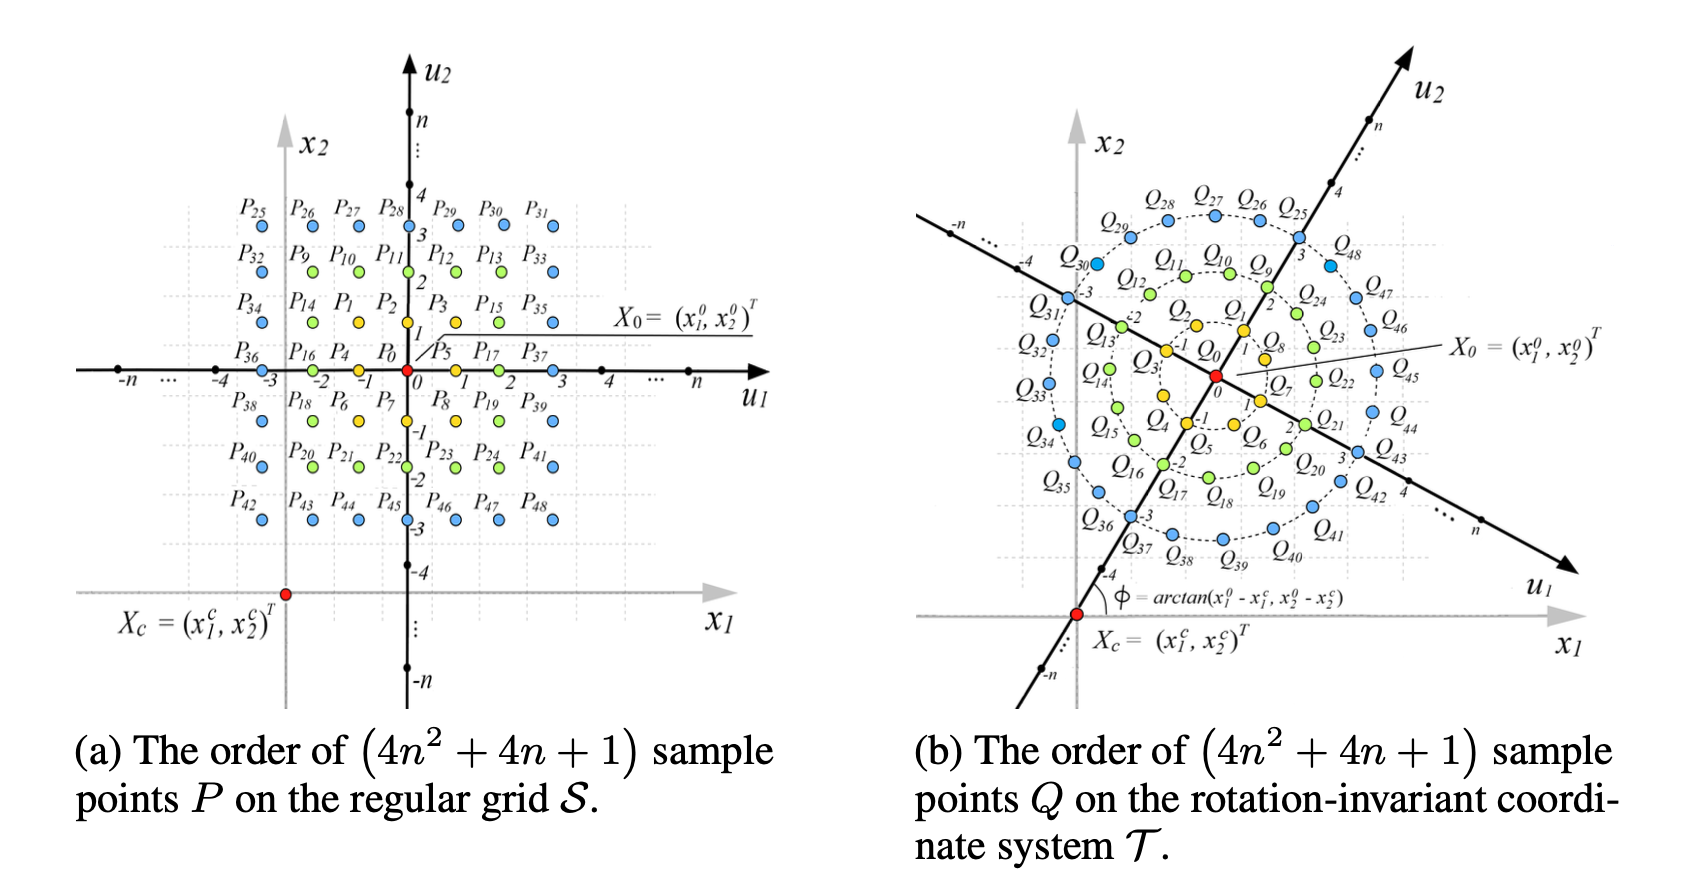
\includegraphics[width=1.0\linewidth]{author-kit-CVPR2025-v3.1-latex-/pics/ric_sample.png}
    \caption{Two sets of sampling points used for calculating $\Phi_C$ and $\Phi_{\mathrm{RIC}-C}$, respectively. It is clear that $Q_\alpha\in\mathcal T$ can be regarded as the corresponding point of $P_\alpha\in\mathcal S$, where $\alpha=0,1,2,\dots,4n^2+4n$.}
    \label{fig:ric_sample}
\end{figure}
RIC-C replaces the fixed grid \(S\) by a \emph{rotation-aware} sampling pattern \(\mathcal T_{X_0}\).  Define
\[
\varphi \;=\;atan2\bigl(x^0_2,\,x^0_1\bigr)
\quad\text{for}\quad
X_0=(x^0_1,x^0_2)^T
\]
and let the kernel cover radii \(r=1,\dots,n\).  On each circle of radius \(r\), sample
\begin{equation}
Q_{r,i}
=
\bigl(r\cos(\varphi + \tfrac{2\pi\,i}{8r}),\,r\sin(\varphi + \tfrac{2\pi\,i}{8r})\bigr),
\quad
i=0,1,\dots,8r-1.
\label{eq:ric_points}
\end{equation}
Collecting all such \(Q_{r,i}\) (plus the center \(Q_{0}=(0,0)\)) defines
\(\;\mathcal T_{X_0}=\{Q_{r,i}\}\).
The RIC-C operation is then
\begin{equation}
\Phi_{\mathrm{RIC\text{-}C}}(X_0, F)
\;=\;
\sum_{Q \,\in\, \mathcal T_{X_0}} W(Q)\,F(X_0 + Q).
\label{eq:ric_conv}
\end{equation}

\noindent
Because \(\mathcal T_{X_0}\) itself rotates by the same angle when the input is rotated about the image center, one can show
\(\Phi_{\mathrm{RIC\text{-}C}}(Y_0,G) = \Phi_{\mathrm{RIC\text{-}C}}(X_0,F)\)
for any rotation \(G(Y) = F(R_{-\theta} Y)\), proving invariance. In \ref{fig:ric_sample}, the sampling scheme of each method can be compared.

\subsubsection*{Key Limitations}

\begin{itemize}
  \item \textbf{Loss of Orientation Information.}  Enforcing full invariance discards absolute angle cues, making it hard to distinguish classes that differ only by rotation (e.g.\ ‘6’ vs.\ ‘9’).  
  \item \textbf{Center-Only Invariance.}  The proof assumes rotations about the image (or feature-map) center; arbitrary pivot points are not covered.  
  \item \textbf{Interpolation \& Pooling Artifacts.}  Sampling at fractional coordinates requires interpolation (e.g.\ bilinear), and subsequent max-pooling layers are not strictly equivariant, leading to small but accumulative errors.
\end{itemize}
\section{Methodology}
\label{sec:method}

In this section, we describe the three methods we employ to combine CNNs and RIC-CNNs:
%-------------------------------------------------------------------------
\subsection{Double Branch Model}

In this approach, we create a network with two branches: one with a standard CNN architecture, and the other with a RIC-CNN architecture. The idea is to allow each branch to learn different aspects of the input image. The CNN branch learns the detailed features, and the RIC-CNN branch learns the rotationally invariant features. The outputs of the two branches are then combined to make the final prediction.  In our implementation, the RIC-CNN branch is frozen for the first few epochs of training. This allows the CNN branch to initially learn basic features without being influenced by the RIC-CNN branch.

%-------------------------------------------------------------------------
\subsection{Take Best Confidence}

This approach is based on the intuition that when a rotated image is passed through a standard CNN, the CNN may not recognize the pattern if it has not seen that specific rotation during training. This leads to a more spread-out confidence score across different classes, resulting in a lower peak confidence.  RIC-CNN, on the other hand, is expected to produce a more reliable prediction with a higher peak confidence due to its rotational invariance.
\\ \\
Similarly, when an unrotated image is passed through an RIC-CNN, examples like label 6 and 9 in MNIST will look the same for RIC-CNN because of its rotational invariance property. This leads to a more spread-out confidence score across these classes, resulting in a lower peak confidence. In this case, standard CNN can clearly distinguish the difference between these labels and give more concentrated and higher peak confidence compared to RIC-CNN.
\\ \\
Therefore, in this approach, we take the prediction with the highest confidence score from either the CNN or the RIC-CNN to be the output.


%-------------------------------------------------------------------------
\subsection{Feature Fusion}

RIC–CNN’s intermediate feature maps are rotation-equivariant: when the input is rotated, the RIC branch’s feature map $F_r$ rotates correspondingly before global averaging. In contrast, a standard CNN’s feature map $F_c$ remains rotationally variant. This mismatch between $F_r$ and $F_c$ encodes rich rotational information. To harness this, we propose a \emph{Feature Fusion} module that compares and dynamically weights these two feature maps to extract and leverage rotational cues for improved robustness.

\subsubsection{Notation}
Let $F_r\in\mathbb{R}^{H\times W\times C}$ be the feature map produced by the RIC branch and $F_c\in\mathbb{R}^{H\times W\times C}$ the feature map from the standard CNN branch at the same spatial resolution and channel dimensionality.

\subsubsection{Weight Generation}
We concatenate the two feature maps along the channel dimension and pass them through a $1\times1$ convolutional layer $g(\cdot)$, followed by a sigmoid activation to produce a spatially-varying weight map:
\[
W = \sigma\bigl(g([F_r \| F_c])\bigr),
\]
where $[\cdot\|\cdot]$ denotes channel-wise concatenation and $\sigma$ is the element-wise sigmoid.

\subsubsection{Fused Representation}
The fused feature map $F_f$ is computed as a per-pixel interpolation of $F_r$ and $F_c$:
\[
F_f = W \odot F_r + (1 - W) \odot F_c,
\]
where $\odot$ denotes broadcasted element-wise multiplication. In regions where the RIC branch’s rotation-equivariant features are more informative, $W$ approaches 1; elsewhere, the standard CNN features dominate.

\subsubsection{Auxiliary Supervision}
To encourage each branch to learn discriminative features, we attach auxiliary classifiers $h_r(\cdot)$ and $h_c(\cdot)$ to $F_r$ and $F_c$, respectively. The final classification is performed by $h_f(F_f)$. The overall loss is:
\[
\mathcal{L} = \mathcal{L}_{\mathrm{CE}}\bigl(h_f(F_f), y\bigr) + \lambda_r \, \mathcal{L}_{\mathrm{CE}}\bigl(h_r(F_r), y\bigr) + \lambda_c \, \mathcal{L}_{\mathrm{CE}}\bigl(h_c(F_c), y\bigr),
\]
where $\mathcal{L}_{\mathrm{CE}}$ is the cross-entropy loss, $y$ the ground-truth label, and $\lambda_r,\lambda_c$ balance the auxiliary terms.

This fusion mechanism dynamically extracts rotational information from the mismatch between equivariant and variant feature maps, leading to balanced performance on both rotated and non-rotated inputs.
\section{Results}
\label{sec:results}

In this section, we present the results of our experiments on the MNIST and Traffic Signs datasets.

\subsection{MNIST Dataset}
Our experiments on the MNIST dataset demonstrate the effectiveness of our proposed methods in handling rotated digits. 
The Double Branch model, Take Best Confidence, and Feature Fusion approaches all show improved performance compared to a standard CNN. 
In particular, the Feature Fusion method achieves the best results, demonstrating the benefit of combining both rotation-invariant and rotation-equivariant features.
The results are shown in \cref{fig:mnist_results}.

\begin{figure}
    \centering
    \includegraphics[width=0.5\linewidth]{pics/mnist_results.png}
    \caption{Results on the MNIST dataset.}
    \label{fig:mnist_results}
\end{figure}


\subsection{Traffic Signs Dataset}
The Traffic Signs dataset presents a more complex challenge due to the presence of rotational symmetries in some signs. Our methods also show promising results on this dataset. Notably, the Feature Fusion method again outperforms the other approaches, highlighting its ability to effectively handle images with more complex rotational properties. The results on the Traffic Signs dataset also confirm that our methods improve the robustness of CNNs to rotation in more complex, real-world scenarios.
{
    \small
    \bibliographystyle{ieeenat_fullname}
    \bibliography{main}
}

% WARNING: do not forget to delete the supplementary pages from your submission 
% \clearpage
\setcounter{page}{1}
\maketitlesupplementary


\section{Rationale}
\label{sec:rationale}
% 
Having the supplementary compiled together with the main paper means that:
% 
\begin{itemize}
\item The supplementary can back-reference sections of the main paper, for example, we can refer to \cref{sec:intro};
\item The main paper can forward reference sub-sections within the supplementary explicitly (e.g. referring to a particular experiment); 
\item When submitted to arXiv, the supplementary will already included at the end of the paper.
\end{itemize}
% 
To split the supplementary pages from the main paper, you can use \href{https://support.apple.com/en-ca/guide/preview/prvw11793/mac#:~:text=Delete%20a%20page%20from%20a,or%20choose%20Edit%20%3E%20Delete).}{Preview (on macOS)}, \href{https://www.adobe.com/acrobat/how-to/delete-pages-from-pdf.html#:~:text=Choose%20%E2%80%9CTools%E2%80%9D%20%3E%20%E2%80%9COrganize,or%20pages%20from%20the%20file.}{Adobe Acrobat} (on all OSs), as well as \href{https://superuser.com/questions/517986/is-it-possible-to-delete-some-pages-of-a-pdf-document}{command line tools}.

\end{document}
